\documentclass[tikz,border=5pt]{standalone}
\usepackage{tikz}
\usepackage{amssymb}
\usetikzlibrary{arrows.meta}
\begin{document}
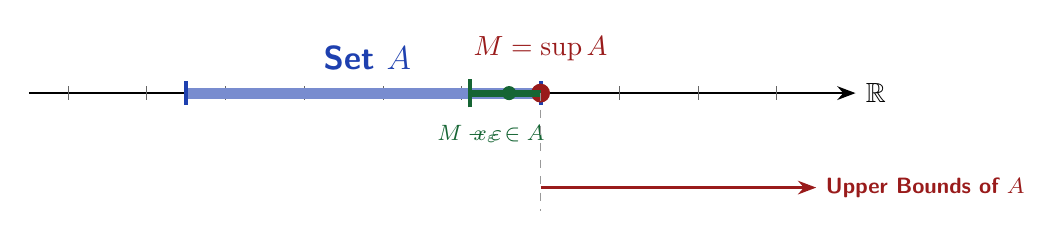
\begin{tikzpicture}[>=Stealth, scale=1.0]
  \definecolor{setblue}{HTML}{1E40AF}
  \definecolor{forestgreen}{HTML}{166534}
  \definecolor{accentcrimson}{HTML}{991B1B}

  % Real number line
  \draw[thick, ->] (-4.5,0) -- (6.0,0) node[right, font=\sffamily\bfseries] {$\mathbb{R}$};
  \foreach \x in {-4,-3,-2,-1,0,1,2,3,4,5}
    \draw[shift={(\x,0)}, color=black!60] (0pt,2.5pt) -- (0pt,-2.5pt);

  % Set A
  \draw[line width=4pt, setblue!60] (-2.5,0) -- (2.0,0);
  \node[setblue, font=\sffamily\bfseries\large] at (-0.2, 0.45) {Set $A$};
  \draw[line width=1.5pt, setblue] (-2.5,-0.15) -- (-2.5,0.15);
  \draw[line width=1.5pt, setblue] (2.0,-0.15) -- (2.0,0.15);

  % Supremum M
  \draw[thick, accentcrimson, fill=accentcrimson] (2.0,0) circle (3pt);
  \node[above=8pt, accentcrimson, font=\sffamily\bfseries] at (2.0,0) {$M = \sup A$};

  % Epsilon interval (M - epsilon, M]
  \draw[line width=2.5pt, forestgreen] (1.1,0) -- (2.0,0);
  \draw[line width=1.5pt, forestgreen] (1.1,-0.18) -- (1.1,0.18);
  \node[below=8pt, forestgreen, font=\sffamily\footnotesize\bfseries] at (1.1,0) {$M - \varepsilon$};

  \node[circle, fill=forestgreen, inner sep=1.8pt] at (1.6,0) {};
  \node[below=8pt, forestgreen, font=\sffamily\footnotesize\bfseries] at (1.6,0) {$x_\varepsilon \in A$};

  % Upper bounds region
  \draw[thick, ->, accentcrimson] (2.0, -1.2) -- (5.5, -1.2);
  \node[right, accentcrimson, font=\sffamily\footnotesize\bfseries] at (5.5, -1.2) {Upper Bounds of $A$};
  \draw[dashed, black!40] (2.0, 0) -- (2.0, -1.5);
\end{tikzpicture}
\end{document}